\documentclass[16pt]{article}
\usepackage[a4paper, margin=2cm]{geometry}
\usepackage{amsmath}
\usepackage{graphicx}
\usepackage{multicol}
\usepackage{multirow}
\title{CSE 300: Online Assignment}
\author{Md Shamsuzzoha Bayzid, Mahjabin Nahar, Md Shariful Islam Bhuyan,\\ 
    and Md Saidur Rahman}
\date{June 2021}

\begin{document}
    \maketitle
    \section{Introduction}
    This assignment has been designed to assess the preparation of the students in writing scientific articles using \LaTeX. This assignment covers a variety of components that are commonly used in scientific manuscripts.
    \subsection{Equations}
    Let $a_0$, $a_n$ and $b_n$ are terms of a series. Their definitions are given by Eqn. 1.\\
    \vspace{2em}
    \begin{align}
        a_0=\frac{1}{\pi}\int_{-\pi}^{\pi}f(x)\,dx\notag\\
        a_n=\frac{1}{\pi}\int_{-\pi}^{\pi}f(x)\cos{nx}\,dx=\frac{1}{\pi}\int_{-\pi}^{\pi}x^2\cos{nx}dx\notag\\
        b_n=\frac{1}{\pi}\int_{-\pi}^{\pi}f(x)\sin{nx}dx=\frac{1}{\pi}\int_{-\pi}^{\pi}x^2\sin{nx}dx\notag\\
    \end{align}
    \subsection{Tables}
        We wish to place the Table at the bottom of the page.
    \subsection{Figures}
        We intend to put Figure 1 at the top of a page.
        \newpage
        \begin{table}[t]
            \centering
            \begin{tabular}{cc}
            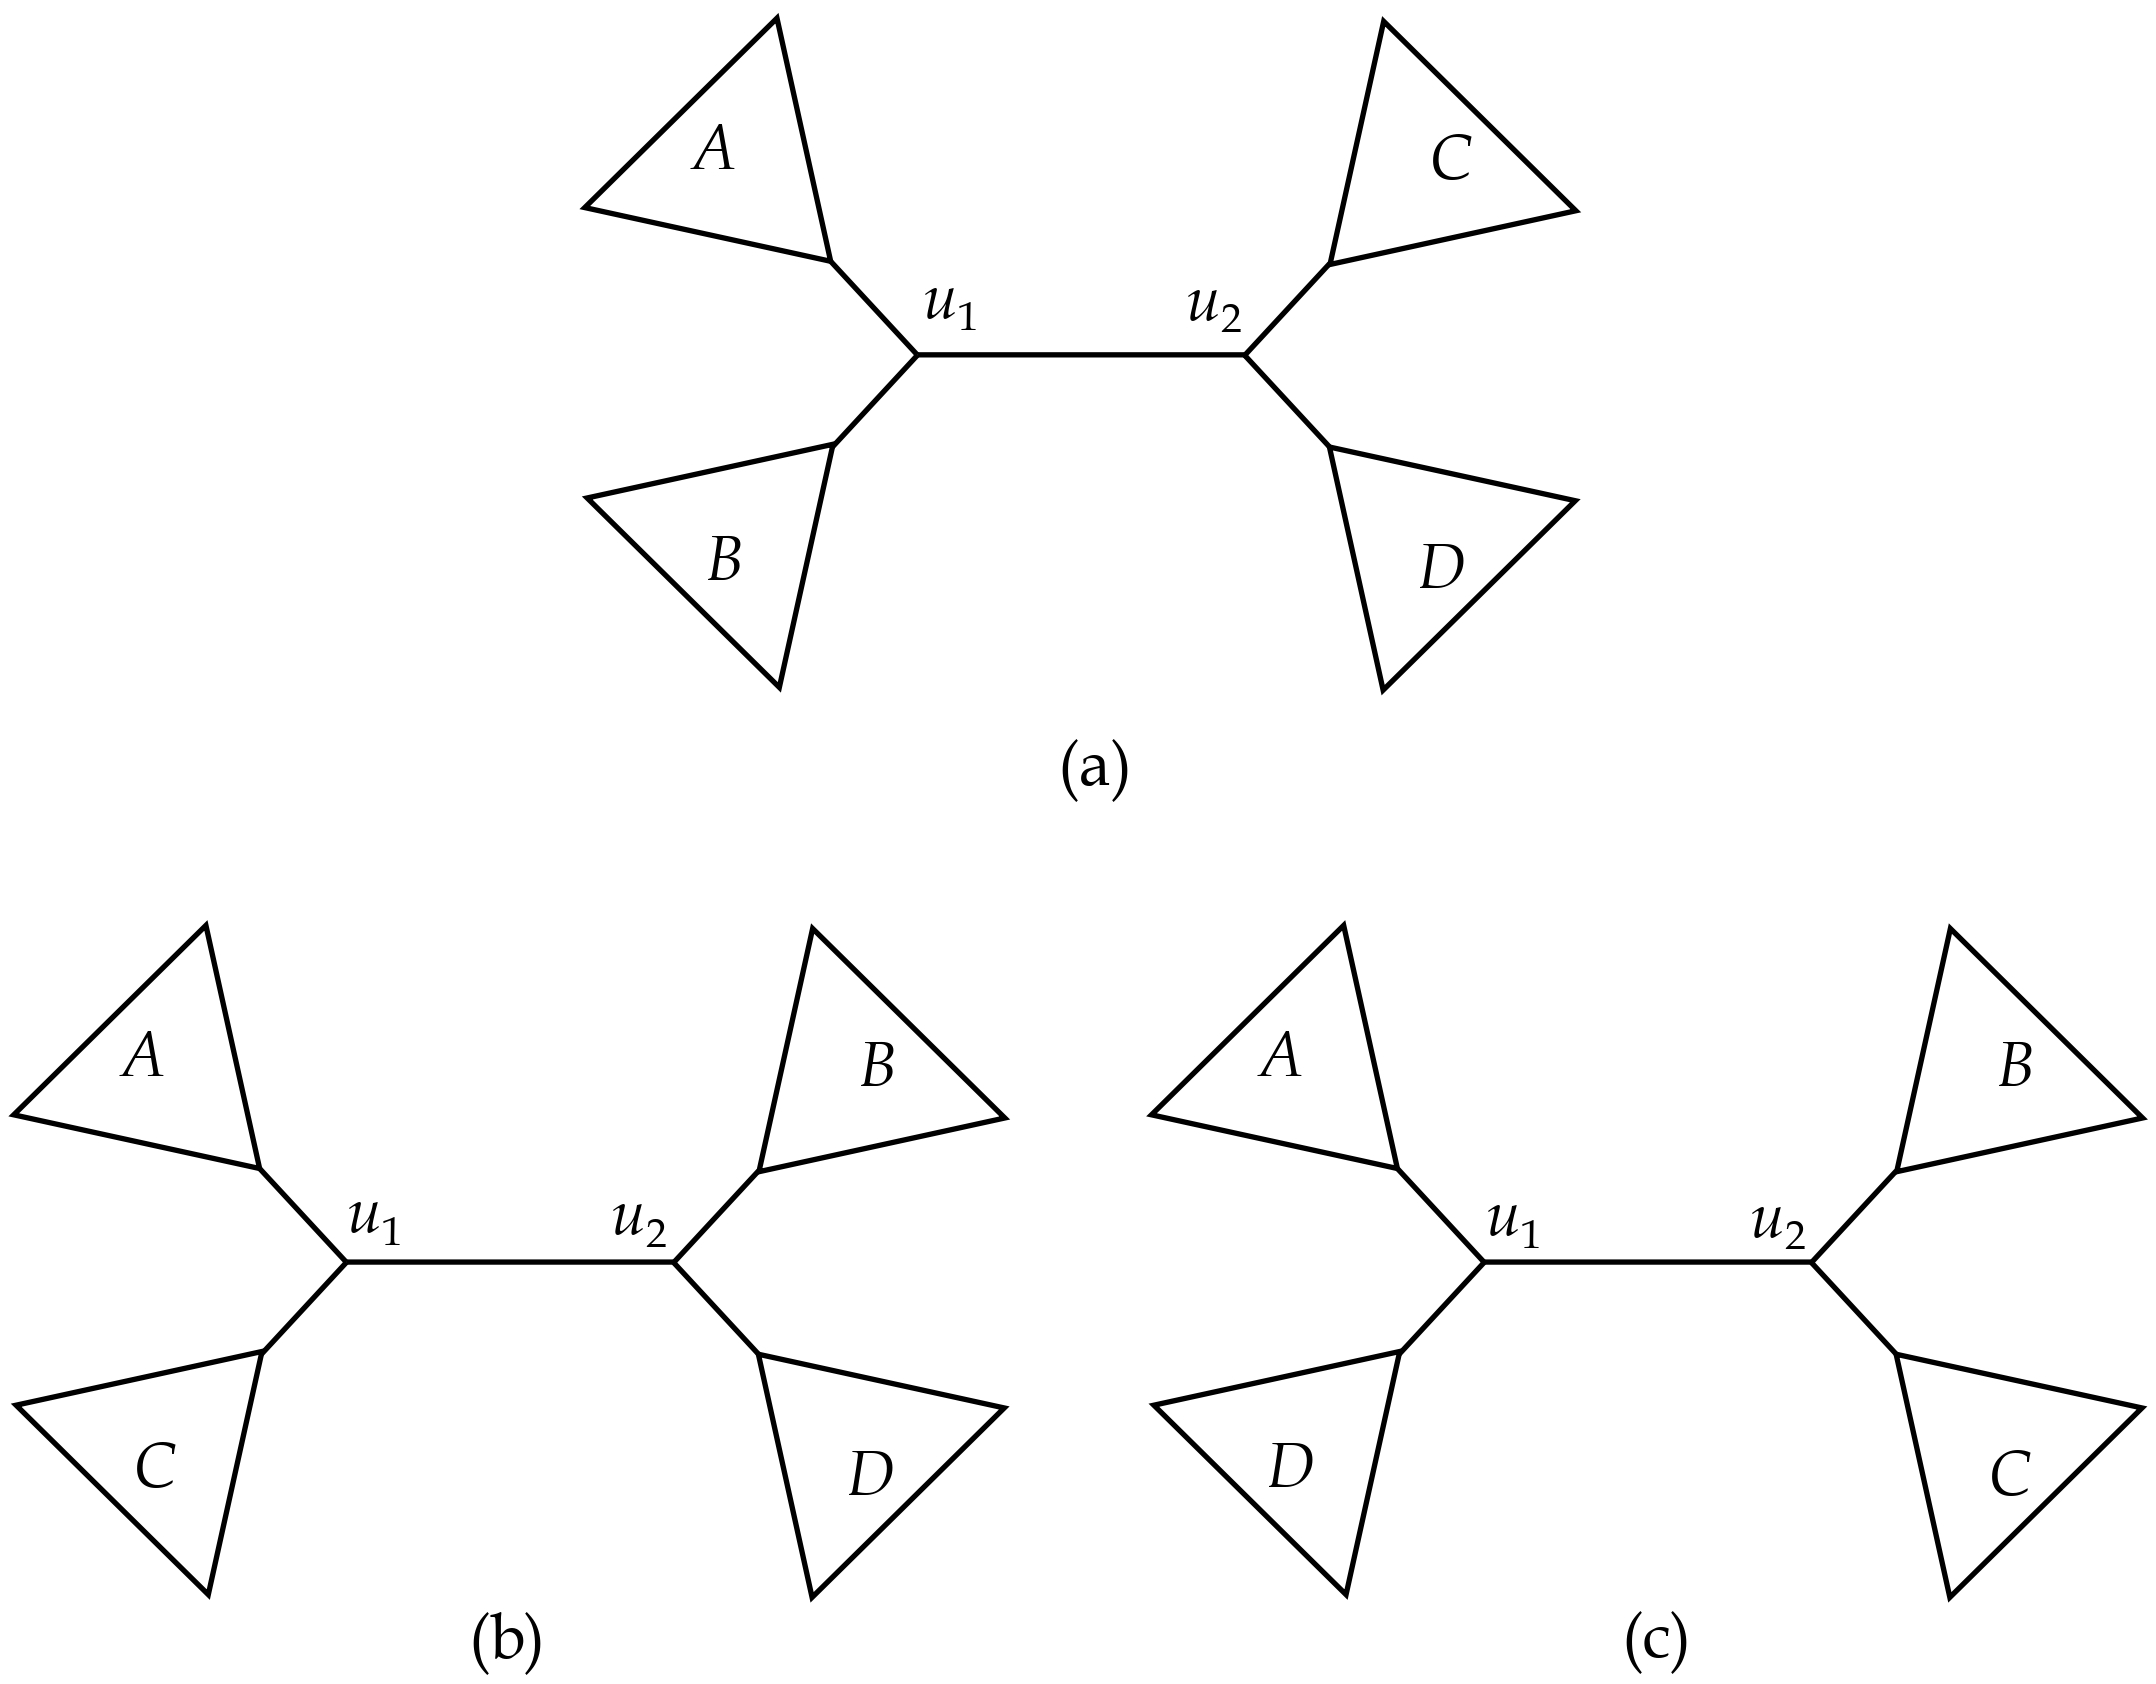
\includegraphics[scale=0.25, angle=90]{Images/Practice_Problem_1_Figure_page-0001.jpg}
            &         
            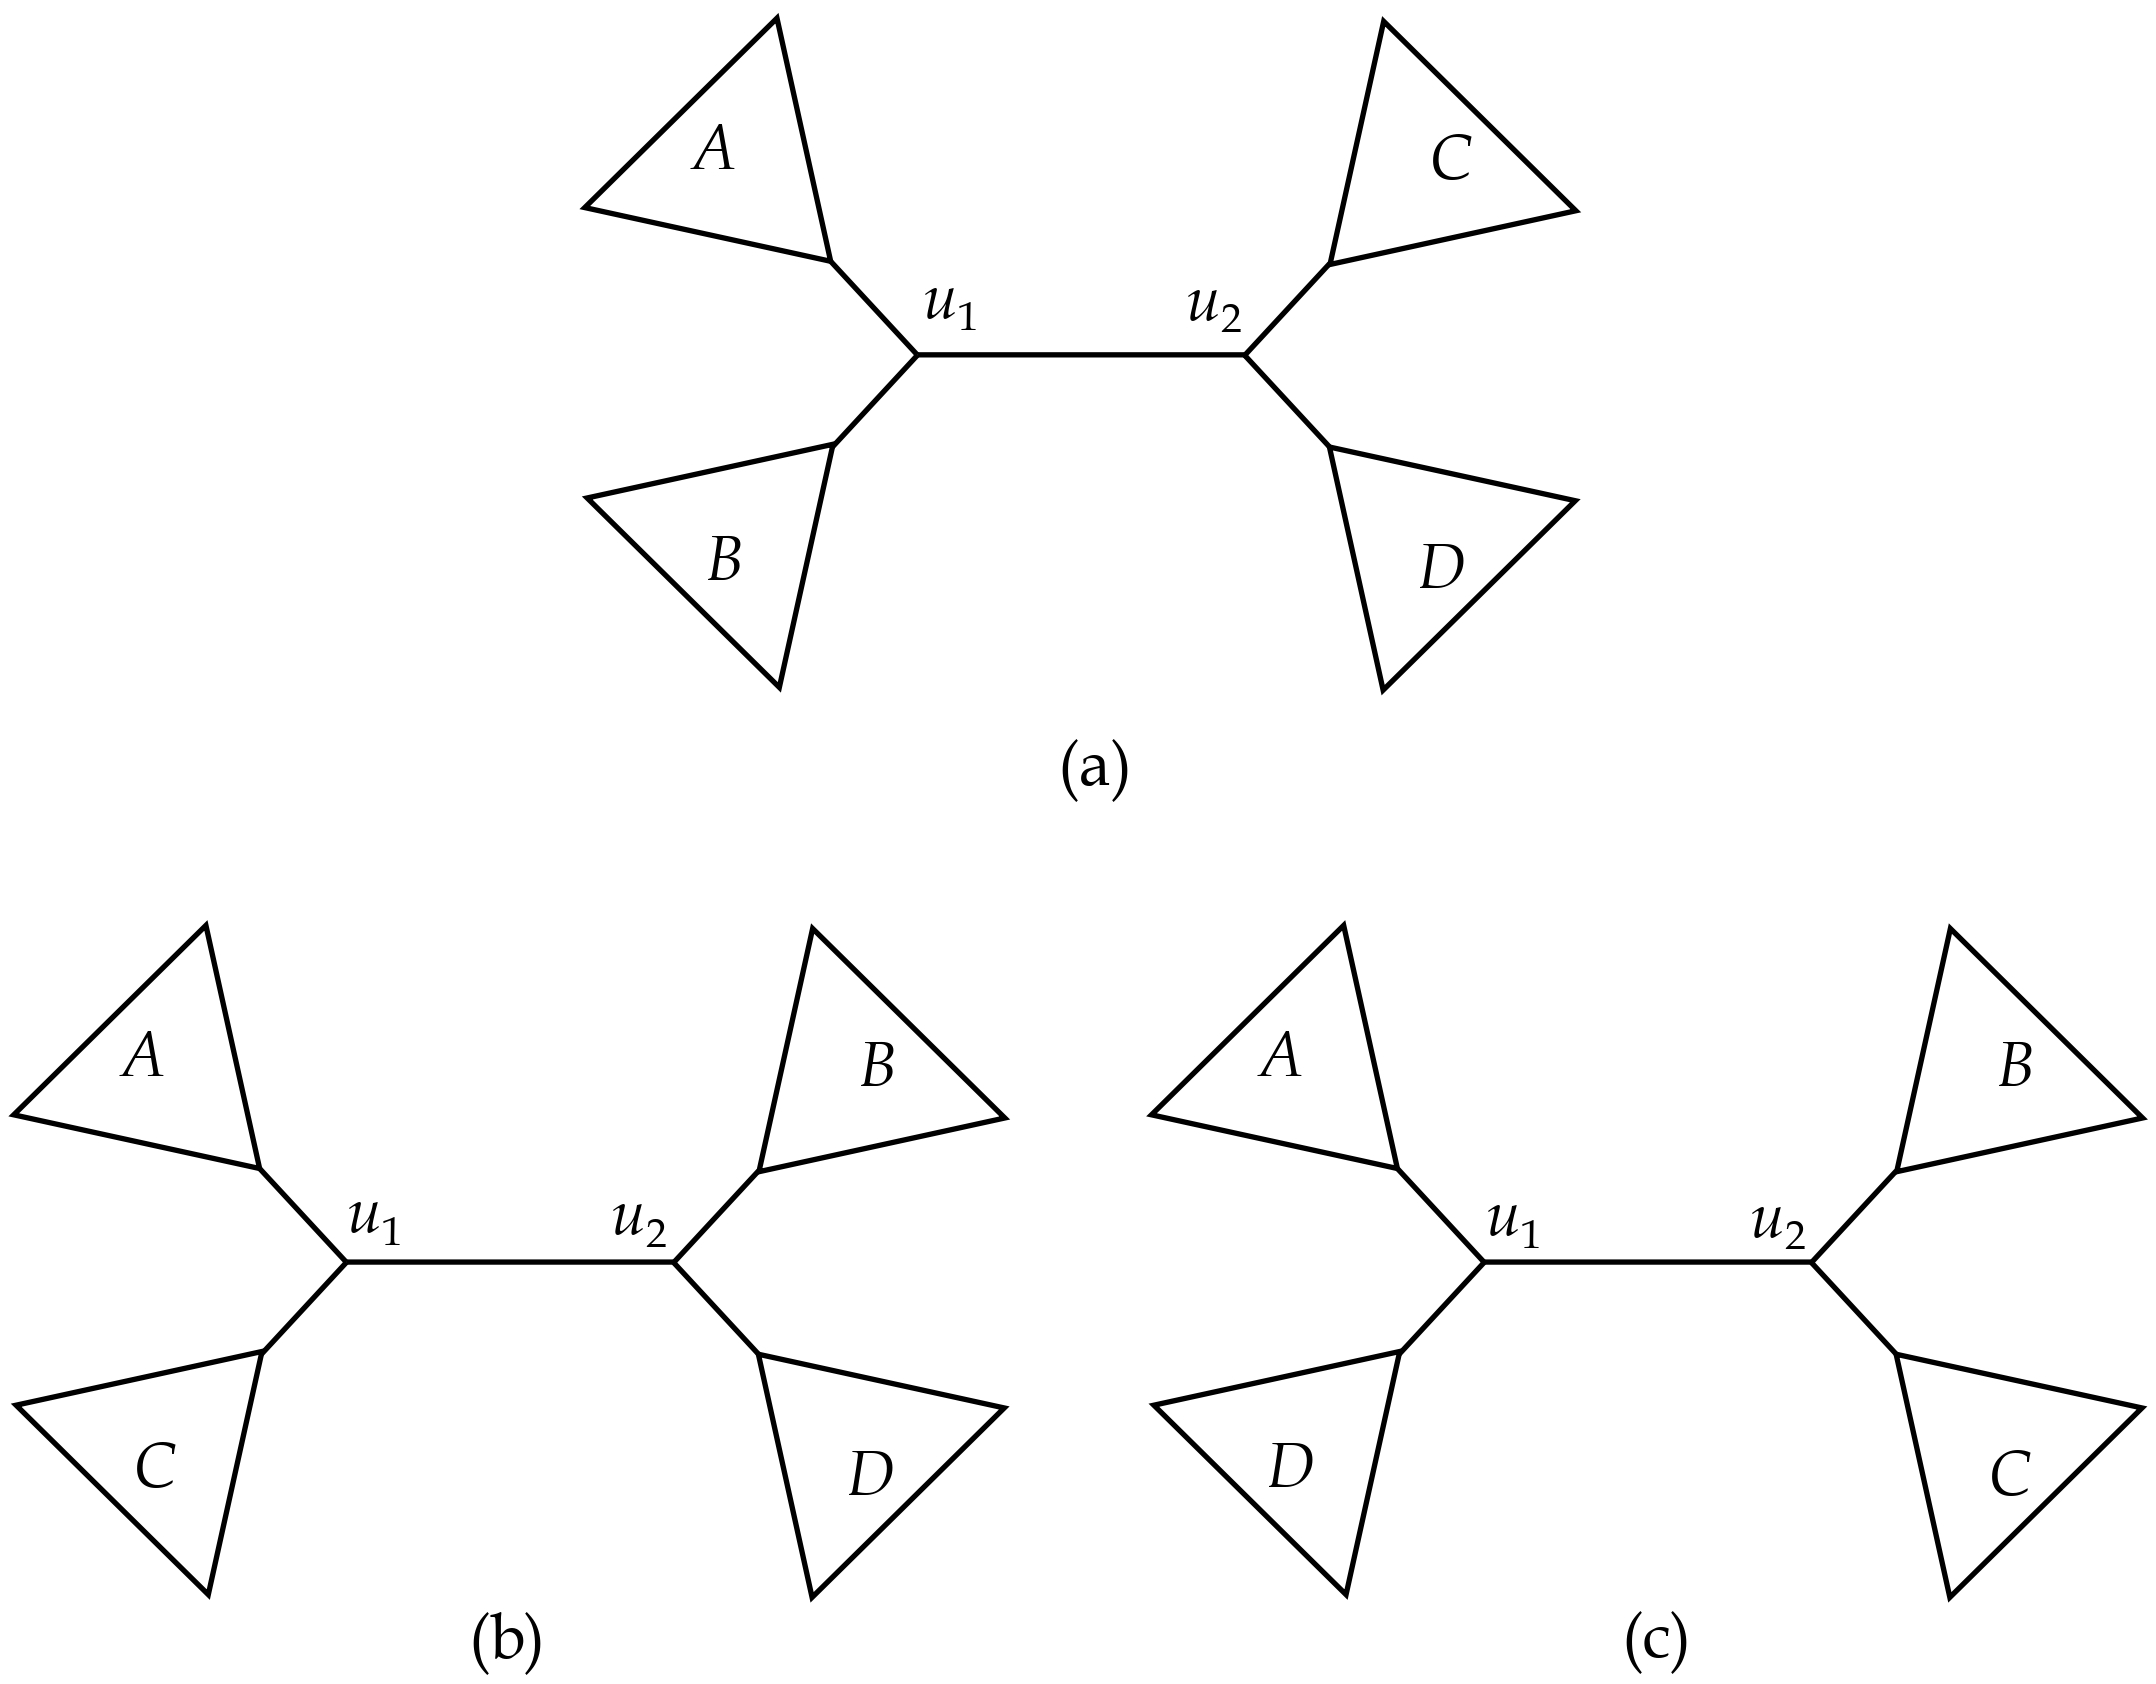
\includegraphics[scale=0.25, angle=90]{Images/Practice_Problem_1_Figure_page-0001.jpg}\\
            \multicolumn{2}{c}{}\\
            \multicolumn{2}{c}{Figure 1: \textbf{Side by side same figure}}
            \end{tabular}
            \label{tab:my_label1}
        \end{table}
    \section{Conclusion}
    The major objectives of this assignment are listed below (please do not ignore\\ the font sizes).
    \begin{itemize}
        \item \large To assess the ability of the students in preparing\\ manuscripts in \LaTeX.
        \item \large To see if the students have adequately practiced different\\ aspects of writing in \LaTeX
    \end{itemize}
    \begin{table}[b]
        \centering
        \begin{tabular}{|c|c|c|c|}
        \hline
        \multicolumn{4}{|c|}{Item List}\\ 
        \hline
        Item Name or & \multirow{2}{*}{ALPHA 2 Code} & \multirow{2}{*}{ALPHA 3 Code} & \multirow{2}{*}{Numeric Code} \\
        Product Name & & &\\
        \hline
        Item001 & AF & AFG & 
        \multirow{4}{*}{
            \begin{tabular}{|c|c|c|c}
                \cline{1-1}
                004 & \multicolumn{3}{c}{}\\
                \cline{1-1}
                \cline{1-1}
                008 & \multicolumn{3}{c}{}\\
                \cline{1-1}
                \cline{1-1}
                009 & \multicolumn{3}{c}{}\\
                \cline{1-1}
                \cline{1-3}
                012 & 013 & 014 &\\
                \cline{1-3}
            \end{tabular}}\\
        Item002 & AX & ALA &\\
        Item003 & AL & ALB &\\
        Item004 & DZ & DZA &\\
        \hline
        \hline
        Item005 & AS & ASM & 
        \multirow{3}{*}{
            \begin{tabular}{|c|c|c|c}
                \cline{1-1}
                016 & \multicolumn{3}{c}{}\\
                \cline{1-1}
                \cline{1-2}
                010 & 020 & \multicolumn{2}{c}{}\\
                \cline{1-2}
                \cline{1-2}
                024 & 025 & \multicolumn{2}{c}{}\\
                \cline{1-2}
            \end{tabular}}\\
        Item006 & AD & AND &\\
        Item007 & AO & AGO &\\
        \hline
        \hline
        \hline
        \end{tabular}
    \end{table}
    \newpage
    \begin{itemize}
        \item To see if the students can add various basic components (e.g., tables, figures, equations) to a \LaTeX \hspace{1em} manuscript.
        \item To see if the students can leverage the available materials (both offline and online) to do something which has not explicitly been taught in the class.
    \end{itemize}
    
    
\end{document}